\documentclass[11pt,a4paper]{article}
\usepackage{xeCJK}
\setmainfont{Times New Roman}
\setsansfont{Helvetica Neue}
\setmonofont{Menlo}
\setCJKmainfont{STSong}
\setCJKsansfont{Heiti TC}
\usepackage[a4paper,margin=24mm,headheight=14pt]{geometry}
\usepackage{amsmath}
\DeclareMathSizes{11}{11}{10}{10}
\DeclareMathSizes{10}{10}{10}{10}
\DeclareMathSizes{9}{10}{10}{10}
\usepackage{booktabs,tabularx,enumitem,xcolor,graphicx,listings,tikz,hyperref,fancyhdr}
\usetikzlibrary{arrows.meta,positioning,calc}
\definecolor{navy}{HTML}{214B63}
\definecolor{codebg}{HTML}{F1F5F7}
\hypersetup{colorlinks=true,linkcolor=navy,urlcolor=navy,pdftitle={从 Bank Conflict 到 GEMM 数据搬运},pdfauthor={KuangjuX}}
\pagestyle{fancy}\fancyhf{}\lhead{GPU 编程笔记}\rhead{KuangjuX}\cfoot{\thepage}
\setlength{\parindent}{2em}\setlength{\parskip}{0.45em}
\lstset{language=C++,basicstyle=\ttfamily\small,backgroundcolor=\color{codebg},frame=single,framerule=0pt,breaklines=true,columns=fullflexible,xleftmargin=5mm,xrightmargin=5mm}
\newenvironment{correction}{\begin{quote}\color{navy}\small\textbf{校注：}}{\end{quote}}
\newcommand{\paperfigure}[3][.72]{%
  \par\medskip\noindent
  \begin{minipage}{\linewidth}\centering
    \includegraphics[width=#1\linewidth]{#2}\par\smallskip
    \refstepcounter{figure}{\small 图 \thefigure：#3}
  \end{minipage}\par\medskip
}
\begin{document}
\begin{titlepage}\centering\vspace*{18mm}{\bfseries GPU MEMORY · TECHNICAL ESSAY}\par\vspace{12mm}
{\Huge\bfseries 从 Bank Conflict 到 GEMM 数据搬运\par}\vspace{5mm}
{\Large 共享内存冲突、Swizzle 与全局内存到寄存器的数据路径\par}\vfill
{\large KuangjuX\par}\vspace{3mm}{\large 2026 年 9 月排印版\par}\vspace{20mm}
\begin{minipage}{0.82\textwidth}\small
本文从共享内存 Bank Conflict 与 Swizzle 出发，继续分析 GEMM 中从全局内存到共享内存、再到寄存器的数据搬运流程。正文仅修正明显的文字、代码标点错误；对涉及硬件语义且容易引起误解的表述，以“校注”单独说明。
\end{minipage}
\end{titlepage}
\tableofcontents
\clearpage

想写一篇文章写一下关于 Bank Conflict 与 Swizzle 的问题，我被这个问题折磨了很久，虽然知乎上有这么多文章，但还是希望写一篇来梳理一下思路。

\section{Bank Conflict}

一个当前最常见的应用场景就是矩阵乘的时候从共享内存到寄存器的内存拷贝操作会涉及到 Bank Conflict 的问题。在 NVIDIA GPU 中一个 Cache line 的大小为 128 Bytes，即为 1024 bits。而每个 Cache line 中分为多个 Banks。当一个线程访问超过 4 bytes（32 bits），即每个 warp 超过 128 bytes（1024 bits）的时候，GPU 不会发出单个事务（transaction），每个事务的最大为 128 bytes。如果每个线程按照向量化访问最大 16 bytes（128 bits）进行访问时，那个 warp wide 将为 512 bytes，此时 GPU 会将其分解为 4 个事务，其中 T0--T7，T8--T15，T16--T23，T24--T31 分别产生一个事务，每个事务的宽度为 128 bytes。Bank Conflict 将按照事务产生而并非按照请求或者 warp、指令产生。

\begin{quote}\itshape
The determination of bank conflicts is made per transaction, not per request or per warp or per instruction.
\end{quote}

当产生 Bank Conflict 的时候，内存访问由并行访问变成串行访问，会极大地影响性能。

\begin{correction}
原文用“Cache line”帮助描述 128-byte 的访问范围。这里需要把三个概念分开：共享内存 bank、一次 warp 指令提出的请求，以及硬件为完成该请求实际执行的 transaction。共享内存并不存在一个与全局内存缓存完全相同的“128 B cache line”；128 B 在这段讨论中用于描述事务拆分的范围。

对计算能力 5.x 及之后的常见 NVIDIA 架构，共享内存有 32 个 bank，每个 bank 每个时钟可提供 32 bit 带宽，连续的 32-bit word 依次映射到连续 bank。若以 byte address $a$ 表示地址，可用
\[
\operatorname{bank}(a)=\lfloor a/4\rfloor\bmod 32
\]
分析映射。因此两个地址相差 128 B 时，bank 编号重新回绕到同一位置，因为 $128/4=32$。这解释了图中 T0/T4 等访问为什么可能落到相同 bank，但是否真正发生冲突，还必须确认它们属于同一个 transaction，并且访问的是同一 bank 中的不同 word。

若多个线程读取完全相同的共享内存 word，硬件可以广播该 word，这不按普通 bank conflict 处理。反之，同一 transaction 内若多个线程访问同一 bank 的不同 word，请求会被拆成若干个无冲突的步骤串行完成。因而判断冲突的可靠方法是：先按指令实际产生的 transaction 分组，再在每组内检查 bank 编号与 word 地址，而不是只看整个 warp 的总字节数。
\end{correction}

在安培架构中，当一块内存希望被从共享内存加载到寄存器内存中，通常会使用硬件提供的 \texttt{ldmatrix} 指令，此时一个线程会加载 128 bits 数据并将其分散到寄存器文件的四个角上面，如下图所示。

\paperfigure[.72]{figures/bank-ldmatrix-clean.png}{从共享内存加载数据到寄存器文件}

然而，当八个线程对第一个 $8\times8$ 的矩阵块进行 \texttt{ldmatrix} 将会造成 Bank Conflict。如下图所示，一个 $16\times16$ 的矩阵块在物理角度看来是一个 $32\times8$ 的块，其中一行为一个 Cache line 的大小。因此当 T0 与 T4 进行数据访问的时候将会发生 Bank Conflict，同理 T1 与 T5，T2 与 T6，T3 与 T7 也是一样的。因此，为了避免 Bank Conflict 的情况，需要避免 8 个线程对相同的 Bank 进行访问的情况。在上面我们了解到 Bank Conflict 总是发生在一个事务内，因此接下来我们只需考虑 T0--T7 这个过程中的 Bank Conflict 的问题即可，而不必关注整个 Warp 内的所有线程，同时 T8--T15，T16--T23，T24--T31 同理。

\par\medskip\noindent
\begin{minipage}{\linewidth}\centering
\resizebox{.80\linewidth}{!}{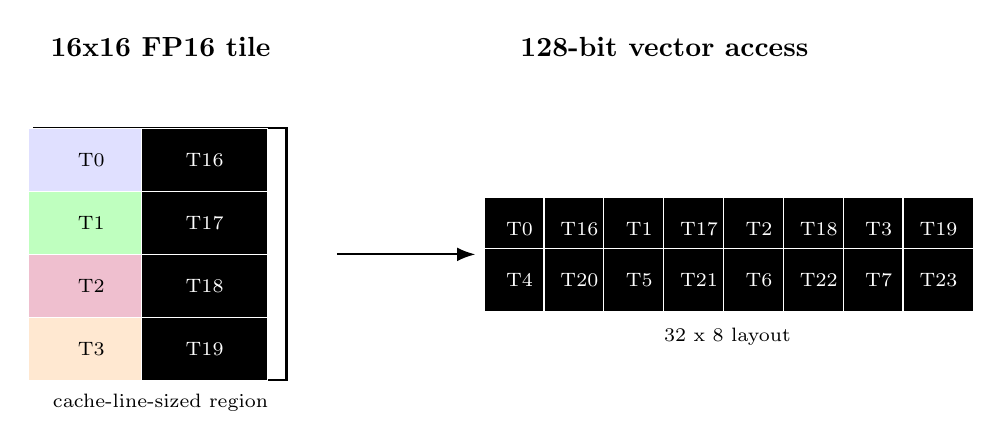
\begin{tikzpicture}[x=8mm,y=8mm,>=Latex]
\node[font=\bfseries] at (2,5.3) {16x16 FP16 tile};
\draw[thick] (0,0) rectangle (4,4);
\node[fill=blue!12!white,draw=white,minimum width=16mm,minimum height=8mm,font=\scriptsize] at (.9,3.5) {T0};\node[fill=black,draw=white,minimum width=16mm,minimum height=8mm,font=\scriptsize,text=white] at (2.7,3.5) {T16};
\node[fill=green!25!white,draw=white,minimum width=16mm,minimum height=8mm,font=\scriptsize] at (.9,2.5) {T1};\node[fill=black,draw=white,minimum width=16mm,minimum height=8mm,font=\scriptsize,text=white] at (2.7,2.5) {T17};
\node[fill=purple!25!white,draw=white,minimum width=16mm,minimum height=8mm,font=\scriptsize] at (.9,1.5) {T2};\node[fill=black,draw=white,minimum width=16mm,minimum height=8mm,font=\scriptsize,text=white] at (2.7,1.5) {T18};
\node[fill=orange!18!white,draw=white,minimum width=16mm,minimum height=8mm,font=\scriptsize] at (.9,.5) {T3};\node[fill=black,draw=white,minimum width=16mm,minimum height=8mm,font=\scriptsize,text=white] at (2.7,.5) {T19};
\node[font=\scriptsize] at (2,-.35) {cache-line-sized region};
\draw[->,thick] (4.8,2)--(7,2);
\node[font=\bfseries] at (10,5.3) {128-bit vector access};
\draw[thick] (7.2,1.2) rectangle (14.8,2.8);
\foreach \i/\name in {0/T0,1/T16,2/T1,3/T17,4/T2,5/T18,6/T3,7/T19}{\node[fill=black,draw=white,minimum width=9mm,minimum height=8mm,font=\scriptsize,text=white] at (7.7+\i*.95,2.4) {\name};}
\foreach \i/\name in {0/T4,1/T20,2/T5,3/T21,4/T6,5/T22,6/T7,7/T23}{\node[fill=black,draw=white,minimum width=9mm,minimum height=8mm,font=\scriptsize,text=white] at (7.7+\i*.95,1.6) {\name};}
\node[font=\scriptsize] at (11,0.7) {32 x 8 layout};
\end{tikzpicture}}\par\smallskip
\refstepcounter{figure}{\small 图 \thefigure：从共享内存加载时发生 Bank Conflict}
\end{minipage}\par\medskip

一种可行的方法是使用 Padding，通过向内存中填充无用的空白数据来使得内存错位，从而避免 Bank Conflict 的问题。例如，下图中通过向共享内存中第一行 Cache line 末尾插入了一段空白内存，在这种情况下，原本由 T19 访问的数据被转移到了下一个 Cache line 中，从而使得 T0/T4，T1/T5，T2/T6，T3/T7 能够在不同 Bank 进行访问，避免了 Bank Conflict。然而，Padding 的缺点在于会过多占用内存，同时也会产生未对齐地址。

\paperfigure[.84]{figures/swizzle-padding-redrawn.png}{Padding 与 Swizzle 的内存布局}

\clearpage
\section{Swizzle}
\begingroup
\small
\setlength{\parskip}{0.25em}

当前较为流行的方式是使用 Swizzle 来对不同的块重新进行物理映射，通过重映射的方式，能够将本来在相同 Bank 的内存映射到不同的物理地址，但对于用户来说逻辑地址依然为原来的地址。

在 CUTLASS 中给了一个通用的 Swizzle 计算方法，定义了 B，M，S 三个符号并通过一系列变换公式来对 Layout 进行重映射。其中 M 表示为一个 Swizzle 重映射的最小单元，在 $2^M\times16$ bits 的数据中的所有数据之间的顺序不会产生变化，这是基于 NVIDIA 中向量化访问考虑的，一次向量化访问最大可访问 128 bits。S 表示基于 M 构成的进行一次内存重映射的元素个数，表示对 $2^S$ 个块在一行内进行重排序。B 表示构成整个 Swizzle 二维空间的行数。

例如 \texttt{Swizzle<B, M, S> = Swizzle<3, 3, 3>} 表示每 128 bits 组成一个块，一行有 8 个块，共有 8 行。当规定完成后，即可对共享内存中二维数组的编号进行重映射，在 Swizzle 中采用行列坐标进行异或的方式进行物理内存重映射。之所以采用异或的原因在于异或操作满足封闭性与双射性，同时经过验证后发现这种方式可以满足 Bank Conflict free 的要求。

\begin{correction}
CUTLASS/CuTe 中的 $B$、$M$、$S$ 首先是地址位字段参数，而不是二维矩阵的三个形状参数。$B$ 表示参与 XOR 的位宽，$M$ 表示不参与重排的低位数，$S$ 表示源位字段与目标位字段之间的距离。它们只有和基础 Layout、地址计量单位以及元素类型合在一起，才能解释成图中的行、列或块。

对于 $S\ge B$，若 $x$ 是 Swizzle 接收的整数偏移量，映射可写为
\[
y=(x\gg(M+S))\mathbin{\&}(2^B-1),\qquad x'=x\mathbin{\oplus}(y\ll M).
\]
以 \texttt{Swizzle<3,3,3>} 为例，最低的 3 bit 保持不变；更高处的 3 bit 被取出，并 XOR 到紧邻低位字段的 3 bit 上。若这里的偏移单位是 FP16 元素，那么保持不变的 $2^3=8$ 个元素正好占 16 B；但“16 B 小块”是由元素类型与偏移单位共同得到的，并不是模板参数本身固定代表 16 B。

原文所说的 $8\times8$ 行列 XOR，是基础 Layout 恰好把一组“行索引位”放到源字段、把一组“列块索引位”放到目标字段时形成的直观解释。在这种映射中，每一行会选择一个不同的列块排列。XOR 映射具有双射性，而且对相同掩码再次 XOR 可以恢复原地址，所以不会丢失或重复元素；但它并不对任意 Layout 自动保证 bank-conflict free。最终是否无冲突，仍取决于元素大小、基础 Layout、每个线程的访问向量，以及一次 transaction 中实际出现的地址集合。
\end{correction}

因此，接下来我们可以对坐标进行重映射计算。

对于第一行：
\[
(0,0):0\oplus0=0,\qquad (0,1):0\oplus1=1,\qquad \ldots,\qquad (0,7):0\oplus7=7.
\]

对于第一行的坐标，行坐标为 0，列坐标为 0--7，异或后与列坐标相同。

对于第二行：
\[
\begin{aligned}
(1,0)&:1\oplus0=1, & (1,1)&:1\oplus1=0,\\
(1,2)&:1\oplus2=3, & (1,3)&:1\oplus3=2,\\
&& (1,7)&:1\oplus7=6.
\end{aligned}
\]

经过 Swizzle 后的内存映射如上图所示，此时可以看见 T0/T4、T1/T5、T2/T6、T3/T7 之间的内存访问完全把 Bank 分开进行访问，此时前八个线程的内存访问达到了 Bank Conflict free。其他线程的访问同理可以避免 Bank Conflict，在这种情况下 Swizzle 可以实现 Bank Conflict free。在此时尽管对于物理地址的访问发生了变化，但对于用户来说逻辑地址依然是不变的。

CUTLASS 中对于 Swizzle 的实现包含在 \href{https://github.com/NVIDIA/cutlass/blob/main/include/cute/swizzle.hpp}{\texttt{include/cute/swizzle.hpp}} 文件中。
\endgroup

\clearpage
\section{GEMM 内存拷贝全流程}

在前文中我们介绍了 Bank Conflict 以及如何使用 Swizzle 来避免 Bank Conflict。在下文中我希望更进一步分析内存拷贝的全流程分析，即内存是如何一步步从全局内存拷贝到共享内存以及寄存器的。本文依然使用应用最广的通用矩阵乘作为示例进行说明。

\paperfigure[.82]{figures/gemm-overview-clean.png}{完整 GEMM 数据拷贝流程}

上图展示了一个 GEMM 从全局内存到共享内存再到寄存器文件中的全部流程。接下来本文将以 A 矩阵的加载为例分析全流程内存拷贝情况。首先 A 矩阵被定义为一个布局为 $[M,K]$ 的行主序矩阵，随后该矩阵将被切块加载到共享内存中并从共享内存加载到寄存器内存中。

\subsection{Global To Shared}

首先全局内存将会按照行列进行切块，本文假设全局内存按照 $[kTM,kTK]$ 的维度对 A 矩阵进行切块，并按照 K 维度进行切分，其中一个 Block 将处理一个大小为 $[kTM,kK]$ 的块。对于 CuTe 编程较为熟悉的话可以得知该内存布局可以被表示为：

\begin{lstlisting}
using GmemLayoutA = Layout<
    Shape<Int<kTM>, Int<kTK>>,
    Stride<Int<kK>, _1>>;
\end{lstlisting}

其中 \texttt{kK} 作为一个 Stride 进行表示。随后一个大小为 $[kTM,kTK]$ 的块被加载入共享内存，下图展示了这一流程。

\paperfigure[.64]{figures/global-shared-clean.png}{从全局内存加载到共享内存}

在从全局内存中加载到共享内存的过程中，为了满足内存合并访问以及方便更进一步从共享内存到寄存器内存的数据搬运，这需要重新对共享内存的 Layout 进行 reshape。在 CuTe 中提供了一个名为 \texttt{cute::tile\_to\_shape} 的函数能够将一个 Layout 复制到更大的形状中（类似于 \texttt{numpy.tile} 操作）。因此，接下来可以将一块大小为 $[kTM,kTK]$ 的内存进行重新切分并 reshape。这在 CuTe 中可以如下表示：

\begin{lstlisting}
using SmemLayoutA = decltype(tile_to_shape(
    SmemLayoutAtom{}, Shape<Int<kTM>, Int<kTK>>{}));
\end{lstlisting}

SmemLayoutA 表示使用 SmemLayoutAtom 作为一个基础块并平铺成一个大小为 $[kTM,kTK]$ 的块。其中 SmemLayoutA 的选择需要综合考虑全局内存与寄存器内存的特性。在一次 FP16 的 \texttt{ldmatrix.x4} 从共享内存到寄存器内存中的加载过程中，需要搬运的数据量为 $16\times16=256$ 个 FP16 的数据。因此，一个 SmemLayoutAtom 的选择应该以 256 作为基础，这将会有多个选择，例如 $16\times16$、$8\times32$、$4\times64$ 等。为了确定哪种 SmemLayoutAtom 更好，更进一步需要考虑的是全局内存的合并内存访问。

\begin{correction}
\texttt{ldmatrix.sync.aligned.m8n8.x4.shared.b16} 是一条 warp 级协作指令：32 个线程共同从共享内存装载四个 $8\times8$、元素宽度为 16 bit 的矩阵。四个矩阵合计包含 $4\times8\times8=256$ 个 16-bit 元素，也就是 512 B；对 \texttt{x4} 形式，每个 lane 接收四个 32-bit 目的寄存器，共 16 B。这里的“256 个元素”描述的是一条 \texttt{ldmatrix.x4} 的总搬运量，不等于 CuTe 中一个 SmemLayoutAtom 必须具有的固定容量。

SmemLayoutAtom 描述的是一个可平铺的共享内存布局原子。它需要同时满足几个约束：CopyAtom 如何把 lane 映射到地址、\texttt{ldmatrix} 所要求的行地址与对齐、共享内存 bank 映射、全局内存写入共享内存时的向量宽度，以及后续 MMA fragment 期望的数据排列。地址由不同 lane 组提供，并不意味着 LayoutAtom 的边界必须与一次 \texttt{ldmatrix.x4} 的 512 B 覆盖范围重合。

因此，$16\times16$、$8\times32$ 或 $4\times64$ 都可以作为“256 元素形状”的候选直觉，但不能仅凭元素总数判断优劣。实际设计时应把选定 Layout 与线程映射组合起来，分别验证 global-to-shared 的合并访问、shared-to-register 的对齐，以及每个 transaction 内的 bank conflict；最后还要确认寄存器片段能直接供 MMA 指令使用。
\end{correction}

在全局内存中同一个 Warp 中的线程的顺序内存访问可以被分组并作为一次执行，这被称为全局内存合并（Global Memory Coalescing），在优化内核的内存访问以实现峰值带宽时，这是最重要的事情。在 GPU 中支持 32 Bytes、64 Bytes 以及 128 Bytes 的内存访问，因此，假如一个线程加载一个 float（4 B），那么 32 个线程将加载 $4\text{ B}\times32=128\text{ B}$，假如一个 Warp 中的内存访问是连续的，那么所有线程访问将会被合并为一次内存访问。如下图所示：

\paperfigure[.52]{figures/coalescing-clean.png}{全局内存合并访问}

\begin{correction}
对计算能力 6.0 及以上的设备，更准确的分析方式是计算一个 warp 的地址集合覆盖了多少个 32-byte segment；硬件需要相应数量的 32-byte transaction 来服务这些访问。若 32 个线程从 32-byte 对齐地址开始，各自连续读取一个 4-byte float，总覆盖范围为 128 B，因此需要四个 32 B transaction，而不是一个不可再分的 128 B transaction。若起始地址错开 4 B，覆盖范围可能跨越五个 segment，于是需要五个 transaction。

“连续线程访问连续地址”是一种容易得到最少 transaction 的常见模式，但线程编号与地址顺序并不必然要求完全一致。只要地址仍落在相同的四个 32 B segment 中，即使 lane 对这些 word 的访问顺序发生置换，也可能仍只需要四个 transaction。性能还会受到每个 segment 中有效字节比例、缓存命中和重放等因素影响，所以“transaction 数相同”也不等于所有模式的实际吞吐完全相同。

在下文每线程读取 16 B 的例子里，一个完整 warp 一共请求 512 B；若地址连续且对齐，从 32 B 粒度看，理论最少覆盖 16 个 segment。把 8 个线程看成一组 128 B，适合帮助设计线程到向量的映射，但不能据此断言硬件只执行四个 128 B transaction，也不能仅凭 $128/16=8$ 推导 SmemLayoutAtom 的形状。这里讨论的是全局内存合并访问；它与前文共享内存按 bank 检查冲突是两套不同的分析方法。
\end{correction}

回到上述问题，在 GEMM 的示例中，每个线程需要加载 8 个 FP16 数据，即 $8\times2\text{ B}=16\text{ B}$，因此最多可以合并 $128\text{ B}/16\text{ B}=8$ 个线程连续内存访问。即将 SmemLayoutAtom 设置为 $[4,64]$：

\begin{lstlisting}
using SmemLayoutAtom = decltype(composition(
    Swizzle<2, 3, 3>{},
    Layout<Shape<_4, _64>, Stride<_64, _1>>{}));
\end{lstlisting}

另外，在实践过程中使用 $[8,32]$ 的 Layout 似乎也是一个流行的选择。CUTLASS issue \#1051 中也解释了关于 SmemLayoutAtom 的设定含义。接下来就可以将全局内存切块加载到共享内存并进行 reshape。同时，此时需要对 Swizzle 块内内存进行 swizzle，关于 swizzle 的解释已经在前文中进行展示，在这里不再进行赘述。

\paperfigure[.78]{figures/swizzle-padding-redrawn.png}{对共享内存进行 Swizzle}

\subsection{Shared To Reg}

本节将讨论如何将数据从共享内存拷贝到寄存器内存，下图为数据拷贝的图例：

\paperfigure[.64]{figures/shared-registers-clean.png}{从共享内存加载到寄存器内存}

在上一节本文介绍到，从全局内存加载到共享内存需要对切块进行更改 Layout 并进行 reshape，那么从共享内存加载到寄存器内存就将使用 reshape 的 SmemLayoutAtom 作为基础单元进行加载。单个 Warp 基于原子内存进行加载，同时整个共享内存可以基于设定的 WarpLayout 进行并行加载。例如 FlashAttention-2 中对于 Q 矩阵进行切分使用 $[4,1]$ 的 WarpLayout 进行 split：

\paperfigure[.78]{figures/warp-layout-clean.png}{FlashAttention 与 FlashAttention-2 的 Warp 工作划分}

单个 Warp 将一块共享内存使用 \texttt{ldmatrix} 指令加载到寄存器内存中，如下图所示：

\paperfigure[.90]{figures/gemm-ldmatrix-clean.png}{ldmatrix 示例}

同时，这里从共享内存进行访问的过程依然是 Swizzled，即对逻辑 Layout 到物理 Layout 有一个映射，来避免 Bank Conflict 的问题。此时矩阵 A 从全局内存到共享内存再到寄存器内存的拷贝过程就完成了。

\clearpage
\section*{参考资料}
\addcontentsline{toc}{section}{参考资料}
\begin{enumerate}[leftmargin=2em,label={[\arabic*]},itemsep=1em,topsep=1em]
\item \href{https://forums.developer.nvidia.com/t/how-to-understand-the-bank-conflict-of-shared-mem/260900}{NVIDIA Developer Forums: How to understand the bank conflict of shared\_mem.}
\item Bastian Hagedorn et al. \href{https://doi.org/10.1145/3582016.3582018}{Graphene: An IR for Optimized Tensor Computations on GPUs.} ASPLOS 2023.
\item \href{https://github.com/NVIDIA/cutlass}{NVIDIA CUTLASS.}
\item \href{https://developer.nvidia.com/blog/cutlass-linear-algebra-cuda/}{CUTLASS: Fast Linear Algebra in CUDA C++.}
\item \href{https://github.com/TiledTensor/TiledBench/blob/master/benchs/cpp/gemm/cutlass_gemm.cuh}{TiledTensor / TiledBench: cutlass\_gemm.cuh.}
\item \href{https://research.colfax-intl.com/cutlass-tutorial-wgmma-hopper/}{CUTLASS Tutorial: Fast Matrix-Multiplication with WGMMA on NVIDIA Hopper GPUs.}
\item \href{https://siboehm.com/articles/22/CUDA-MMM}{How to Optimize a CUDA Matmul Kernel for cuBLAS-like Performance: a Worklog.}
\item \href{https://github.com/NVIDIA/cutlass/issues/1051}{CUTLASS issue \#1051: How to understand SmemLayoutAtom in CuTe.}
\item Tri Dao. \href{https://arxiv.org/abs/2307.08691}{FlashAttention-2: Faster Attention with Better Parallelism and Work Partitioning.} 2023.
\item \href{https://docs.nvidia.com/cuda/cuda-c-best-practices-guide/}{NVIDIA CUDA C++ Best Practices Guide.}
\item \href{https://docs.nvidia.com/cuda/parallel-thread-execution/index.html#warp-level-matrix-load-instruction-ldmatrix}{NVIDIA PTX ISA: Warp-level matrix load instruction ldmatrix.}
\end{enumerate}

\end{document}
